\chapter{Génétique des populations et sélection naturelle}\label{ch:b2:population-genetics}

En 1848, une phalène du bouleau noire fut capturée près de Manchester~;
en 1895, dix-neuf phalènes sur vingt étaient noires dans la ville, et
vers 1970, à mesure que la suie disparaissait, la forme claire était de
retour. Les phalènes n'avaient pas changé~: les proportions de deux
\omterm{def:b2:meiosis-heredity:vocabulary}{allèles} dans une population de millions d'individus avaient changé, sous
les yeux des oiseaux, en quelques dizaines de générations. Darwin avait
vu que la sélection devait transformer les espèces, mais n'avait aucun
moyen de la chiffrer~; ce chiffrage est la \omterm{def:b2:population-genetics:frequencies}{génétique des populations}, et
c'est l'arithmétique de ce chapitre. Elle se demande comment se
comportent les \omterm{def:b2:population-genetics:frequencies}{fréquences alléliques} lorsque rien n'agit sur elles, puis
à quelle vitesse la sélection, la \omterm{def:b2:genome-diversification:mutation}{mutation}, la migration, le hasard et
la consanguinité les déplacent --- et elle se termine sur les caractères
qui dépendent non d'un gène mais de nombreux gènes, c'est-à-dire la
plus grande partie de ce que la sélection voit réellement.

\section{Le pool génique au repos}

\begin{definition}[Population, pool génique, fréquences]\label{def:b2:population-genetics:frequencies}
\index{genetique des populations@génétique des populations}\index{pool genique@pool génique}\index{frequence allelique@fréquence allélique}
Une \emph{population} est un groupe d'individus d'une même espèce qui se
reproduisent entre eux~; son \emph{pool génique} est l'ensemble de tous
leurs \omterm{def:b2:meiosis-heredity:vocabulary}{allèles}. Pour un locus à deux \omterm{def:b2:meiosis-heredity:vocabulary}{allèles} $A$ et $a$ dans une
population \omterm{def:b2:meiosis-heredity:meiosis}{diploïde} de
$N$ individus, les \emph{fréquences alléliques} sont $p = (2N_{AA} +
N_{Aa})/2N$ et $q = 1 - p$, et les \emph{fréquences génotypiques} sont
les proportions de $AA$, $Aa$ et $aa$. L'évolution, au sens le plus
étroit, est une variation des fréquences alléliques d'une génération à
l'autre~; la question de ce chapitre est de savoir ce qui les fait varier,
et de combien.
\end{definition}

\begin{theorem}[Hardy--Weinberg]\label{thm:b2:population-genetics:hw}
\index{loi de Hardy--Weinberg}
Dans une grande population où les accouplements se font au hasard, sans
sélection, \omterm{def:b2:genome-diversification:mutation}{mutation} ni migration, les \omterm{def:b2:population-genetics:frequencies}{fréquences alléliques} ne varient
pas d'une génération à l'autre, et après une seule génération
d'accouplements au hasard les fréquences génotypiques valent
\[
AA : p^{2}, \qquad Aa : 2pq, \qquad aa : q^{2},
\]
et le restent. La dominance ne fait pas se répandre un \omterm{def:b2:meiosis-heredity:vocabulary}{allèle} \omterm{def:b2:meiosis-heredity:vocabulary}{dominant},
et un \omterm{def:b2:meiosis-heredity:vocabulary}{allèle} \omterm{def:b2:meiosis-heredity:vocabulary}{récessif} rare n'est pas perdu~: il se cache chez les
\omterm{def:b2:meiosis-heredity:vocabulary}{hétérozygotes}, plus nombreux que les \omterm{def:b2:meiosis-heredity:vocabulary}{homozygotes} dans un rapport de
$2p/q$ à un --- pour $q = 0.01$, deux cents contre un. La loi est
l'hypothèse nulle de la \omterm{def:b2:population-genetics:frequencies}{génétique des populations}~: un écart à cette loi
dans une population réelle, ou une variation de
$p$ entre générations, est la signature de l'une des forces décrites
ci-dessous.
\end{theorem}
\begin{proof}
Les accouplements au hasard reviennent à une union au hasard des
gamètes~: un gamète porte $A$ avec la
probabilité $p$ et $a$ avec la probabilité $q$, indépendamment de son
partenaire, si bien que le zygote est $AA$ avec la probabilité $p^{2}$,
$Aa$ avec la probabilité
$2pq$, $aa$ avec la probabilité $q^{2}$. La \omterm{def:b2:population-genetics:frequencies}{fréquence allélique} à la
génération suivante est $p' = p^{2} + \tfrac12(2pq) = p(p + q) = p$~:
inchangée. Comme les fréquences génotypiques ne dépendent que de $p$,
elles sont les mêmes à chaque génération après la première.
\end{proof}

\begin{example}[Lire une fréquence]\label{ex:b2:population-genetics:cf}
La mucoviscidose, récessive, touche un enfant européen sur 2500~:
$q^{2} = 1/2500$, $q = 0.02$, et la fréquence des porteurs est $2pq
\approx 0.04$ --- une personne sur 25 porte un \omterm{def:b2:meiosis-heredity:vocabulary}{allèle} qui tue ses
\omterm{def:b2:meiosis-heredity:vocabulary}{homozygotes}, et \qty{98}{\%} des copies de l'\omterm{def:b2:meiosis-heredity:vocabulary}{allèle} se trouvent chez des
porteurs sains, où la sélection ne peut pas les voir. C'est pourquoi un
\omterm{def:b2:meiosis-heredity:vocabulary}{récessif} létal est éliminé si lentement, et pourquoi les programmes
eugénistes visant à éliminer les maladies récessives en stérilisant les
malades n'auraient jamais pu fonctionner~: l'arithmétique de la section
suivante montre avec quelle lenteur.
\end{example}

\section{La sélection}

\begin{definition}[Valeur sélective]\label{def:b2:population-genetics:fitness}
\index{valeur selective@valeur sélective}\index{coefficient de selection@coefficient de sélection}
La \emph{valeur sélective} $w$ d'un \omterm{def:b2:meiosis-heredity:vocabulary}{génotype} est sa contribution relative
en descendants à la génération suivante --- la survie jusqu'à la
reproduction multipliée par la fécondité, rapportée au meilleur \omterm{def:b2:meiosis-heredity:vocabulary}{génotype},
qui a $w = 1$. Le
\emph{coefficient de sélection} $s$ d'un \omterm{def:b2:meiosis-heredity:vocabulary}{génotype} est son déficit,
$w = 1 - s$. La valeur sélective est une propriété d'un \omterm{def:b2:meiosis-heredity:vocabulary}{génotype} dans un
environnement, non d'un \omterm{def:b2:meiosis-heredity:vocabulary}{allèle} en soi~: l'\omterm{def:b2:meiosis-heredity:vocabulary}{allèle} mélanique de la phalène
avait $w > 1$ par rapport à l'\omterm{def:b2:meiosis-heredity:vocabulary}{allèle} clair sur une \omterm{def:b2:plant-meristems:wood}{écorce} couverte de
suie et $w < 1$ sur les lichens.
\end{definition}

\begin{theorem}[La sélection modifie la fréquence allélique]\label{thm:b2:population-genetics:selection}
\index{selection naturelle@sélection naturelle!equation@équation}
Avec des \omterm{def:b2:population-genetics:fitness}{valeurs sélectives} génotypiques $w_{AA}$, $w_{Aa}$, $w_{aa}$, la
\omterm{def:b2:population-genetics:fitness}{valeur sélective} moyenne est $\bar w = p^{2}w_{AA} + 2pq\,w_{Aa} + q^{2}w_{aa}$ et la
\omterm{def:b2:population-genetics:frequencies}{fréquence allélique} à la génération suivante vaut
\[
p' = \frac{p^{2}w_{AA} + pq\,w_{Aa}}{\bar w}, \qquad
\Delta p = p' - p = \frac{pq\,\bigl[p(w_{AA} - w_{Aa}) + q(w_{Aa} - w_{aa})\bigr]}{\bar w}.
\]
Deux conséquences. D'abord, $\Delta p$ est proportionnel à $pq$~: la
sélection est la plus rapide aux fréquences intermédiaires et la plus
lente lorsqu'un \omterm{def:b2:meiosis-heredity:vocabulary}{allèle} est rare ou presque fixé --- il y a alors peu de
variation sur laquelle agir.
Ensuite, contre un \omterm{def:b2:meiosis-heredity:vocabulary}{allèle} \omterm{def:b2:meiosis-heredity:vocabulary}{récessif} ($w_{AA} = w_{Aa} = 1$, $w_{aa} =
1 - s$), la variation vaut $\Delta q = -s\,pq^{2}/\bar w$, proportionnelle
à $q^{2}$~: un \omterm{def:b2:meiosis-heredity:vocabulary}{récessif} rare est presque invisible pour la sélection, et
diviser par deux sa fréquence à partir de $0.01$ demande une centaine de
générations, même lorsque ses \omterm{def:b2:meiosis-heredity:vocabulary}{homozygotes} sont létaux. Un \omterm{def:b2:meiosis-heredity:vocabulary}{allèle} \omterm{def:b2:meiosis-heredity:vocabulary}{dominant}
favorable se répand vite au début puis stagne à la fin, pour la même
raison.
\end{theorem}
\begin{proof}
Parmi les descendants, une fraction $p^{2}w_{AA}/\bar w$ sont $AA$ et
$2pq\,w_{Aa}/\bar w$ sont $Aa$ (la fréquence de chaque \omterm{def:b2:meiosis-heredity:vocabulary}{génotype} pondérée
par sa \omterm{def:b2:population-genetics:fitness}{valeur sélective} et renormalisée)~; les \omterm{def:b2:meiosis-heredity:vocabulary}{allèles} $A$ qu'ils portent
sont tous ceux du premier groupe et la moitié de ceux du second, ce qui
donne $p'$. Retrancher $p =
p\bar w/\bar w$ et développer $\bar w$ donne $\Delta p$. Pour un \omterm{def:b2:meiosis-heredity:vocabulary}{récessif}
létal ($s = 1$)~: $q' = q^{2}\cdot 0 + pq$ divisé par $\bar w = 1 -
q^{2}$, donc $q' = q/(1 + q)$, d'où $1/q' = 1/q + 1$ et, au bout de $t$
générations, $1/q_t = 1/q_0 + t$~: passer de $q_0 = 0.01$ à $0.005$ demande
$t = 100$.
\end{proof}

\begin{omfigure}
\begin{tikzpicture}
\begin{axis}[
  width=0.8\linewidth, height=6cm,
  axis x line=bottom, axis y line=left,
  xmin=0, xmax=150, ymin=0, ymax=1.05,
  xlabel={générations}, ylabel={fréquence de l'allèle favorisé},
  xlabel style={font=\small, at={(axis description cs:0.5,-0.11)}, anchor=north},
  ylabel style={font=\small},
  tick label style={font=\small}, xtick={0,50,100,150}, ytick={0,0.5,1},
  legend style={font=\scriptsize, at={(0.97,0.35)}, anchor=east, draw=none},
  clip=false,
]
\addplot[very thick, omDef] table[x=t, y=dom] {
t dom
0 0.01
10 0.02
20 0.04
30 0.075
40 0.14
50 0.24
60 0.38
70 0.53
80 0.66
90 0.76
100 0.83
110 0.88
120 0.91
130 0.93
140 0.945
150 0.955
};
\addlegendentry{allèle favorisé dominant, $s = 0.1$}
\addplot[very thick, omThm] table[x=t, y=rec] {
t rec
0 0.01
10 0.0101
20 0.0102
30 0.0104
40 0.0106
50 0.0108
60 0.011
70 0.0113
80 0.0116
90 0.012
100 0.0124
110 0.0128
120 0.0133
130 0.0138
140 0.0144
150 0.015
};
\addlegendentry{allèle favorisé récessif, $s = 0.1$}
\end{axis}
\end{tikzpicture}

{\small La sélection à l'œuvre avec un avantage de \qty{10}{\%}. Un \omterm{def:b2:meiosis-heredity:vocabulary}{allèle}
\omterm{def:b2:meiosis-heredity:vocabulary}{dominant} favorisé passe de \qty{1}{\%} à la majorité en soixante-dix
générations puis ralentit, son rival \omterm{def:b2:meiosis-heredity:vocabulary}{récessif} rare se cachant chez les
\omterm{def:b2:meiosis-heredity:vocabulary}{hétérozygotes}~; un \omterm{def:b2:meiosis-heredity:vocabulary}{allèle} \omterm{def:b2:meiosis-heredity:vocabulary}{récessif} favorisé à \qty{1}{\%} bouge à peine
dans le même temps, car il n'est presque jamais exposé.}
\end{omfigure}

\begin{proposition}[Les types de sélection]\label{prop:b2:population-genetics:kinds}
\index{selection directionnelle@sélection directionnelle}\index{selection stabilisante@sélection stabilisante}\index{selection balancee@sélection balancée}\index{avantage des heterozygotes@avantage des hétérozygotes}
La sélection \emph{directionnelle} favorise un extrême et entraîne un
\omterm{def:b2:meiosis-heredity:vocabulary}{allèle} vers la fixation (la phalène mélanique dans un bois couvert de
suie~; la résistance aux antibiotiques~; la taille du bec d'un pinson
lors d'une sécheresse).
La sélection \emph{stabilisante} favorise le milieu et élimine les
extrêmes (le poids de naissance humain~: les bébés qui meurent sont les
plus petits et les plus gros)~; elle maintient une population là où elle
est et c'est la plus commune. La sélection \emph{disruptive} favorise les
deux extrêmes contre le milieu, et peut scinder une population
(\cref{ch:b2:speciation}). La sélection \emph{balancée} maintient deux
\omterm{def:b2:meiosis-heredity:vocabulary}{allèles} dans la population indéfiniment~: par \emph{\omterm{prop:b2:population-genetics:kinds}{avantage des
hétérozygotes}}, lorsque $Aa$ a une \omterm{def:b2:population-genetics:fitness}{valeur sélective} supérieure à celle
des deux \omterm{def:b2:meiosis-heredity:vocabulary}{homozygotes} --- avec
$w_{AA} = 1 - s$, $w_{aa} = 1 - t$, $w_{Aa} = 1$, la fréquence
se stabilise à $\hat p = t/(s + t)$ --- ou par sélection
\emph{fréquence-dépendante}, lorsqu'un \omterm{def:b2:meiosis-heredity:vocabulary}{génotype} est d'autant plus avantagé
qu'il est plus rare (les \omterm{def:b2:meiosis-heredity:vocabulary}{allèles}
$S$ rares du \cref{ch:b2:angiosperm-reproduction}, les proies qu'un
prédateur n'a pas appris à reconnaître, les deux côtés de bouche d'un
poisson mangeur d'écailles).
\end{proposition}
\begin{proof}[Faits expérimentaux]
L'hémoglobine drépanocytaire tue la plupart des \omterm{def:b2:meiosis-heredity:vocabulary}{homozygotes} avant qu'ils
se reproduisent, et pourtant l'\omterm{def:b2:meiosis-heredity:vocabulary}{allèle} atteint \qty{10}{\%} à \qty{20}{\%}
dans toute l'Afrique impaludée. Allison (1954) montra que les enfants
\omterm{def:b2:meiosis-heredity:vocabulary}{hétérozygotes} avaient des accès palustres bien moins nombreux et moins
graves que les deux \omterm{def:b2:meiosis-heredity:vocabulary}{homozygotes}, et la fréquence de l'\omterm{def:b2:meiosis-heredity:vocabulary}{allèle} se calque
sur la répartition historique du paludisme à falciparum~; dans les
populations d'ascendance africaine vivant là où il n'y a pas de
paludisme, la fréquence n'a cessé de diminuer depuis. Avec $t \approx 0.8$ pour l'\omterm{def:b2:meiosis-heredity:vocabulary}{homozygote}
drépanocytaire et $s \approx 0.1$ pour l'\omterm{def:b2:meiosis-heredity:vocabulary}{homozygote} normal dans une région
impaludée, $\hat q = s/(s + t) \approx 0.11$ --- ce qu'on observe.
\end{proof}

\section{Mutation, migration et équilibre}

\begin{theorem}[L'équilibre mutation--sélection]\label{thm:b2:population-genetics:balance}
\index{equilibre mutation--selection@équilibre mutation--sélection}\index{fardeau genetique@fardeau génétique}
Un \omterm{def:b2:meiosis-heredity:vocabulary}{allèle} délétère est alimenté par la \omterm{def:b2:genome-diversification:mutation}{mutation} au taux $\mu$ par gamète
et par génération, et éliminé par la sélection. À l'équilibre, les deux
se compensent~: pour un \omterm{def:b2:meiosis-heredity:vocabulary}{allèle} \omterm{def:b2:meiosis-heredity:vocabulary}{récessif} dont le désavantage \omterm{def:b2:meiosis-heredity:vocabulary}{homozygote} vaut $s$,
\[
\hat q = \sqrt{\mu/s}\,;
\]
pour un \omterm{def:b2:meiosis-heredity:vocabulary}{allèle} \omterm{def:b2:meiosis-heredity:vocabulary}{dominant} (ou partiellement \omterm{def:b2:meiosis-heredity:vocabulary}{dominant}) dont le désavantage
\omterm{def:b2:meiosis-heredity:vocabulary}{hétérozygote} vaut $hs$, $\hat q = \mu/hs$. La fréquence d'équilibre d'un
\omterm{def:b2:meiosis-heredity:vocabulary}{récessif} est donc importante, même pour un létal~: avec $\mu = 10^{-5}$ et
$s = 1$, $\hat q = 3\times 10^{-3}$, et \qty{0.6}{\%} de la population
le porte. Toute population porte un tel \emph{\omterm{thm:b2:population-genetics:balance}{fardeau génétique}} en des
milliers de loci, pour l'essentiel \omterm{def:b2:meiosis-heredity:vocabulary}{récessif} et caché, et l'équilibre de
l'argument du cliquet du \cref{ch:b2:asexual-reproduction}
--- une fraction $e^{-U/s}$ d'individus exempts de \omterm{def:b2:genome-diversification:mutation}{mutations}
délétères --- est le même équilibre sommé sur tout le génome.
\end{theorem}
\begin{proof}
À chaque génération, la \omterm{def:b2:genome-diversification:mutation}{mutation} ajoute $\mu p \approx \mu$ à $q$ et la
sélection retire $s\,pq^{2}/\bar w \approx sq^{2}$ (pour $q$ petit)~;
poser $\mu = s\hat q^{2}$ donne le résultat \omterm{def:b2:meiosis-heredity:vocabulary}{récessif}. Pour un \omterm{def:b2:meiosis-heredity:vocabulary}{allèle}
\omterm{def:b2:meiosis-heredity:vocabulary}{dominant}, la sélection retire $hs\,q$ par génération (chaque copie est
exposée chez un \omterm{def:b2:meiosis-heredity:vocabulary}{hétérozygote}), et $\mu = hs\hat q$.
\end{proof}

\begin{proposition}[La migration et la règle d'un migrant]\label{prop:b2:population-genetics:migration}
\index{flux genique@flux génique}\index{migration (genetique)@migration (génétique)}
Si une fraction $m$ d'une population est formée à chaque génération
d'immigrants venus d'une population de \omterm{def:b2:population-genetics:frequencies}{fréquence allélique} $p_{m}$, la
fréquence se rapproche de $p_{m}$ de $\Delta p = m(p_{m} - p)$~: l'écart
entre les deux populations décroît comme $(1 - m)^{t}$. Le \emph{\omterm{prop:b2:population-genetics:migration}{flux
génique}} homogénéise~; il défait l'\omterm{def:b2:plant-plasticity:plasticity}{adaptation} locale à moins que la
sélection ne soit plus forte que $m$, et c'est la force qui maintient une
espèce en une seule espèce. Inversement, des populations qui n'échangent
aucun migrant divergent par dérive et par leurs \omterm{def:b2:genome-diversification:mutation}{mutations} propres, et un
seul migrant par génération --- quelle que soit la taille de la
population --- suffit à les empêcher de dériver jusqu'à la fixation
d'\omterm{def:b2:meiosis-heredity:vocabulary}{allèles} différents.
\end{proposition}

\section{Le hasard~: la dérive génétique}

\begin{theorem}[La dérive génétique]\label{thm:b2:population-genetics:drift}
\index{derive genetique@dérive génétique}\index{effectif efficace}\index{fixation}
Dans une population de $N$ individus \omterm{def:b2:meiosis-heredity:meiosis}{diploïdes}, la \omterm{def:b2:population-genetics:frequencies}{fréquence allélique}
de chaque génération est un échantillon aléatoire de $2N$ gamètes tiré
de la précédente, si bien que $p$ fluctue au hasard avec une variance de
$p(1 - p)/2N$ par génération. L'\emph{hétérozygotie} $H = 2pq$
décroît en moyenne d'un facteur $(1 - 1/2N)$ à chaque génération,
\[
H_t = H_0\left(1 - \frac{1}{2N}\right)^{t} \approx H_0\,e^{-t/2N},
\]
et tout \omterm{def:b2:meiosis-heredity:vocabulary}{allèle} finit par être perdu ou \emph{fixé}, avec une
probabilité égale à sa fréquence actuelle~: une nouvelle \omterm{def:b2:genome-diversification:mutation}{mutation} neutre,
à la fréquence $1/2N$, est fixée avec la probabilité $1/2N$ et, si elle
l'est, met environ $4N$ générations pour y parvenir. La dérive est
négligeable dans une population de millions d'individus et prépondérante
dans une population de quelques dizaines~: un
\emph{goulot d'étranglement} ou un effet \emph{fondateur} --- quelques
colons sur une île, une espèce réduite à une centaine d'individus par la
chasse --- fait perdre des \omterm{def:b2:meiosis-heredity:vocabulary}{allèles} par hasard en une génération et laisse
une population uniforme, appauvrie et riche en \omterm{def:b2:meiosis-heredity:vocabulary}{homozygotes}. Le $N$ qui
compte est l'effectif \emph{efficace}, le nombre d'individus qui se
reproduisent réellement, en général bien inférieur à l'effectif recensé.
\end{theorem}
\begin{proof}
Les $2N$ copies de gènes de la génération suivante sont tirées avec
remise dans un pool où $A$ a la fréquence $p$~: le nombre de copies $A$
suit une loi binomiale de moyenne $2Np$ et de variance $2Np(1 - p)$, donc $p'$ a
pour moyenne $p$ et pour variance $p(1 - p)/2N$. Deux copies tirées au
hasard à la génération suivante proviennent de la même copie parentale
avec la probabilité $1/2N$ et sont alors identiques, si bien que la
probabilité que deux copies diffèrent (l'hétérozygotie) est multipliée
par $1 - 1/2N$ à chaque génération. Probabilité de fixation~: la
fréquence d'un \omterm{def:b2:meiosis-heredity:vocabulary}{allèle} neutre est une martingale --- son espérance ne
change jamais --- et elle finit à 0 ou à 1, donc la probabilité de finir
à 1 est égale à sa valeur de départ.
\end{proof}

\begin{omfigure}
\begin{tikzpicture}
\begin{axis}[
  width=0.82\linewidth, height=6cm,
  axis x line=bottom, axis y line=left,
  xmin=0, xmax=60, ymin=0, ymax=1.05,
  xlabel={générations}, ylabel={fréquence allélique $p$},
  xlabel style={font=\small, at={(axis description cs:0.5,-0.11)}, anchor=north},
  ylabel style={font=\small},
  tick label style={font=\small}, xtick={0,20,40,60}, ytick={0,0.5,1},
  legend style={font=\scriptsize, at={(0.5,-0.25)}, anchor=north, draw=none, legend columns=2},
  clip=false,
]
\addplot[thick, omThm] coordinates {(0,0.5) (2,0.55) (4,0.62) (6,0.58) (8,0.7) (10,0.8) (12,0.75) (14,0.85) (16,0.92) (18,0.88) (20,0.95) (22,1) (60,1)};
\addlegendentry{$N = 10$}
\addplot[thick, omThm!60] coordinates {(0,0.5) (2,0.42) (4,0.35) (6,0.4) (8,0.3) (10,0.2) (12,0.25) (14,0.15) (16,0.1) (18,0.05) (20,0.08) (22,0.02) (24,0) (60,0)};
\addplot[thick, omDef] coordinates {(0,0.5) (5,0.52) (10,0.49) (15,0.53) (20,0.56) (25,0.54) (30,0.58) (35,0.55) (40,0.57) (45,0.6) (50,0.58) (55,0.61) (60,0.6)};
\addlegendentry{$N = 1000$}
\addplot[thick, omDef!60] coordinates {(0,0.5) (5,0.48) (10,0.5) (15,0.47) (20,0.45) (25,0.46) (30,0.44) (35,0.45) (40,0.43) (45,0.44) (50,0.42) (55,0.43) (60,0.42)};
\end{axis}
\end{tikzpicture}

{\small La dérive. Deux populations de dix individus partant de
$p = 0.5$ fixent des \omterm{def:b2:meiosis-heredity:vocabulary}{allèles} opposés en moins de vingt-cinq générations~;
deux populations de mille individus fluctuent de quelques pour cent en
soixante générations.}
\end{omfigure}

\begin{proposition}[La consanguinité]\label{prop:b2:population-genetics:inbreeding}
\index{consanguinite@consanguinité}\index{coefficient de consanguinite@coefficient de consanguinité}\index{depression de consanguinite@dépression de consanguinité}
Les accouplements entre apparentés ne modifient pas les \omterm{def:b2:population-genetics:frequencies}{fréquences
alléliques} mais augmentent la proportion d'\omterm{def:b2:meiosis-heredity:vocabulary}{homozygotes}~: le
\emph{\omterm{prop:b2:population-genetics:inbreeding}{coefficient de consanguinité}} $F$ d'un individu est la probabilité
que ses deux \omterm{def:b2:meiosis-heredity:vocabulary}{allèles} à un locus soient identiques par ascendance, et les
fréquences génotypiques deviennent $p^{2} + Fpq$, $2pq(1 - F)$, $q^{2} + Fpq$. Pour
les enfants de cousins germains $F = 1/16$, de frère et sœur $1/4$,
d'autofécondation $1/2$. Comme les \omterm{def:b2:meiosis-heredity:vocabulary}{allèles} \omterm{def:b2:meiosis-heredity:vocabulary}{récessifs} du \omterm{thm:b2:population-genetics:balance}{fardeau
génétique} sont exposés chez les \omterm{def:b2:meiosis-heredity:vocabulary}{homozygotes} supplémentaires, les
descendants consanguins souffrent de \emph{\omterm{prop:b2:population-genetics:inbreeding}{dépression de consanguinité}}~:
un \omterm{def:b2:meiosis-heredity:vocabulary}{récessif} létal à $q = 0.01$
apparaît chez $q^{2} = 10^{-4}$ des descendants d'accouplements au hasard,
mais chez
$q^{2} + Fpq = 7\times 10^{-4}$ des enfants de cousins, sept fois plus~;
sommée sur des milliers de loci, la mortalité infantile des enfants de
cousins est environ le double de celle des autres, et une petite
population qui se reproduit en consanguinité pendant des générations perd
fertilité et vigueur --- le sort du guépard, de la panthère de Floride et
des maisons royales d'Europe.
\end{proposition}

\section{De nombreux gènes~: les caractères quantitatifs}

\begin{theorem}[L'héritabilité et la réponse à la sélection]\label{thm:b2:population-genetics:heritability}
\index{heritabilite@héritabilité}\index{genetique quantitative@génétique quantitative}\index{equation du selectionneur@équation du sélectionneur}
Un caractère comme la taille, le rendement ou la hauteur du bec est
déterminé par de nombreux gènes à petit effet et par l'environnement, et
varie de façon continue. Sa variance dans une population se décompose en
une part \emph{génétique} $V_G$ et une part \emph{environnementale} $V_E$, et
l'\emph{héritabilité} $h^{2} = V_A/V_P$ est la fraction de la variance
phénotypique due aux effets additifs des gènes (la part qui se
transmet). Si les parents de la génération suivante sont sélectionnés
avec une moyenne qui dépasse celle de la population de $S$ (la
\emph{différentielle de sélection}), leurs descendants la dépassent de
\[
R = h^{2}\,S
\]
--- l'\emph{\omterm{thm:b2:population-genetics:heritability}{équation du sélectionneur}}. C'est toute l'amélioration
animale et végétale en une ligne~: une héritabilité de $0.5$ et des
parents à un écart-type au-dessus de la moyenne donnent des descendants
à un demi-écart-type au-dessus, et le gain s'accumule génération après
génération. L'héritabilité est une propriété d'une population dans un
environnement, non d'un caractère~: elle ne dit rien de la fixité d'un
caractère, et un caractère d'héritabilité $h^{2} = 0.8$ dans une population peut
avoir $h^{2} = 0$ dans une autre, où tous les individus ont le même
\omterm{def:b2:meiosis-heredity:vocabulary}{génotype}.
\end{theorem}
\begin{proof}
Le \omterm{def:b2:meiosis-heredity:vocabulary}{phénotype} attendu des descendants se régresse sur celui du parent
moyen avec une pente $h^{2}$ (la covariance génétique additive entre
apparentés divisée par la variance phénotypique), si bien qu'un écart parental $S$
donne un écart des descendants $h^{2}S$. En pratique, $h^{2}$ se
mesure à partir de cette régression, ou de la ressemblance des jumeaux et
des germains, ou à partir de la réponse elle-même.
\end{proof}
\begin{proof}[Faits expérimentaux]
L'expérience de l'Illinois sur le maïs, commencée en 1896, sélectionna
chaque année les épis les plus riches et les plus pauvres en huile~: au
bout de cent générations, la lignée haute était passée de \qty{5}{\%} à
\qty{20}{\%} d'huile et la lignée basse était tombée sous \qty{1}{\%},
toutes deux répondant encore --- la variation de nombreux gènes n'est pas
épuisée par un siècle de sélection. Aux Galápagos, les Grant mesurèrent
tous les pinsons d'une île pendant la sécheresse de 1977~: les survivants
avaient des becs plus hauts de \qty{4}{\%} que les morts, le caractère
avait une héritabilité $h^{2}
\approx 0.7$, et les oisillons de l'année suivante avaient des becs
plus hauts de \qty{3}{\%} que ceux de la génération précédente --- la
sélection observée, mesurée, et sa réponse prédite par l'équation
ci-dessus.
\end{proof}

\begin{omfigure}
\begin{tikzpicture}
\begin{axis}[
  width=0.78\linewidth, height=5.6cm,
  axis x line=bottom, axis y line=left,
  xmin=6, xmax=14, ymin=0, ymax=0.32,
  xlabel={hauteur du bec (mm)}, ylabel={fréquence},
  xlabel style={font=\small, at={(axis description cs:0.5,-0.12)}, anchor=north},
  ylabel style={font=\small},
  tick label style={font=\small}, xtick={7,9,11,13}, ytick=\empty,
  legend style={font=\scriptsize, at={(0.5,-0.28)}, anchor=north, draw=none, legend columns=3},
  clip=false,
]
\addplot[very thick, omDef, domain=6:14, samples=100] {0.3*exp(-((x-9.4)^2)/(2*0.9))};
\addlegendentry{avant la sécheresse, moyenne 9.4}
\addplot[very thick, omThm, domain=6:14, samples=100] {0.28*exp(-((x-9.9)^2)/(2*0.8))};
\addlegendentry{survivants, moyenne 9.9}
\addplot[very thick, omProp, dashed, domain=6:14, samples=100] {0.3*exp(-((x-9.75)^2)/(2*0.9))};
\addlegendentry{génération suivante, moyenne 9.75}
\draw[<->] (axis cs:9.4,0.02) -- (axis cs:9.9,0.02); \node[font=\scriptsize, anchor=south] at (axis cs:9.65,0.025) {$S$};
\end{axis}
\end{tikzpicture}

{\small L'\omterm{thm:b2:population-genetics:heritability}{équation du sélectionneur} dans une population de pinsons. La
sécheresse a laissé des survivants au bec plus haut en moyenne de
$S = \qty{0.5}{mm}$~; avec
$h^{2} = 0.7$, leurs descendants avaient un bec plus haut de
$R = \qty{0.35}{mm}$ que la génération précédente.}
\end{omfigure}

\begin{example}[L'arithmétique de la phalène]\label{ex:b2:population-genetics:moth}
L'\omterm{def:b2:meiosis-heredity:vocabulary}{allèle} mélanique de la phalène du bouleau est \omterm{def:b2:meiosis-heredity:vocabulary}{dominant}. D'une
fréquence d'environ $10^{-3}$ en 1848 à \qty{90}{\%} de phalènes
mélaniques (une fréquence voisine de $0.7$) en 1895, il y a cinquante
générations~; l'équation de la sélection le reproduit avec $s$ entre $0.2$ et $0.3$ contre la forme claire
--- et les expériences de lâcher de Kettlewell, dans les années 1950,
où les oiseaux prélevaient les phalènes claires sur les troncs couverts
de suie et les sombres sur les troncs propres dans à peu près ce
rapport, mesurèrent directement le coefficient. Le retour après les lois
sur la qualité de l'air, de \qty{90}{\%} de mélaniques en 1960 à
moins de \qty{10}{\%} en 2000, s'est fait à la même vitesse en sens
inverse. L'épisode entier --- une grande population, un \omterm{def:b2:meiosis-heredity:vocabulary}{allèle} \omterm{def:b2:meiosis-heredity:vocabulary}{dominant},
un agent sélectif puissant et réversible --- est la \omterm{def:b2:population-genetics:frequencies}{génétique des
populations} en train de se faire sous les yeux de tous.
\end{example}

\begin{omfigure}
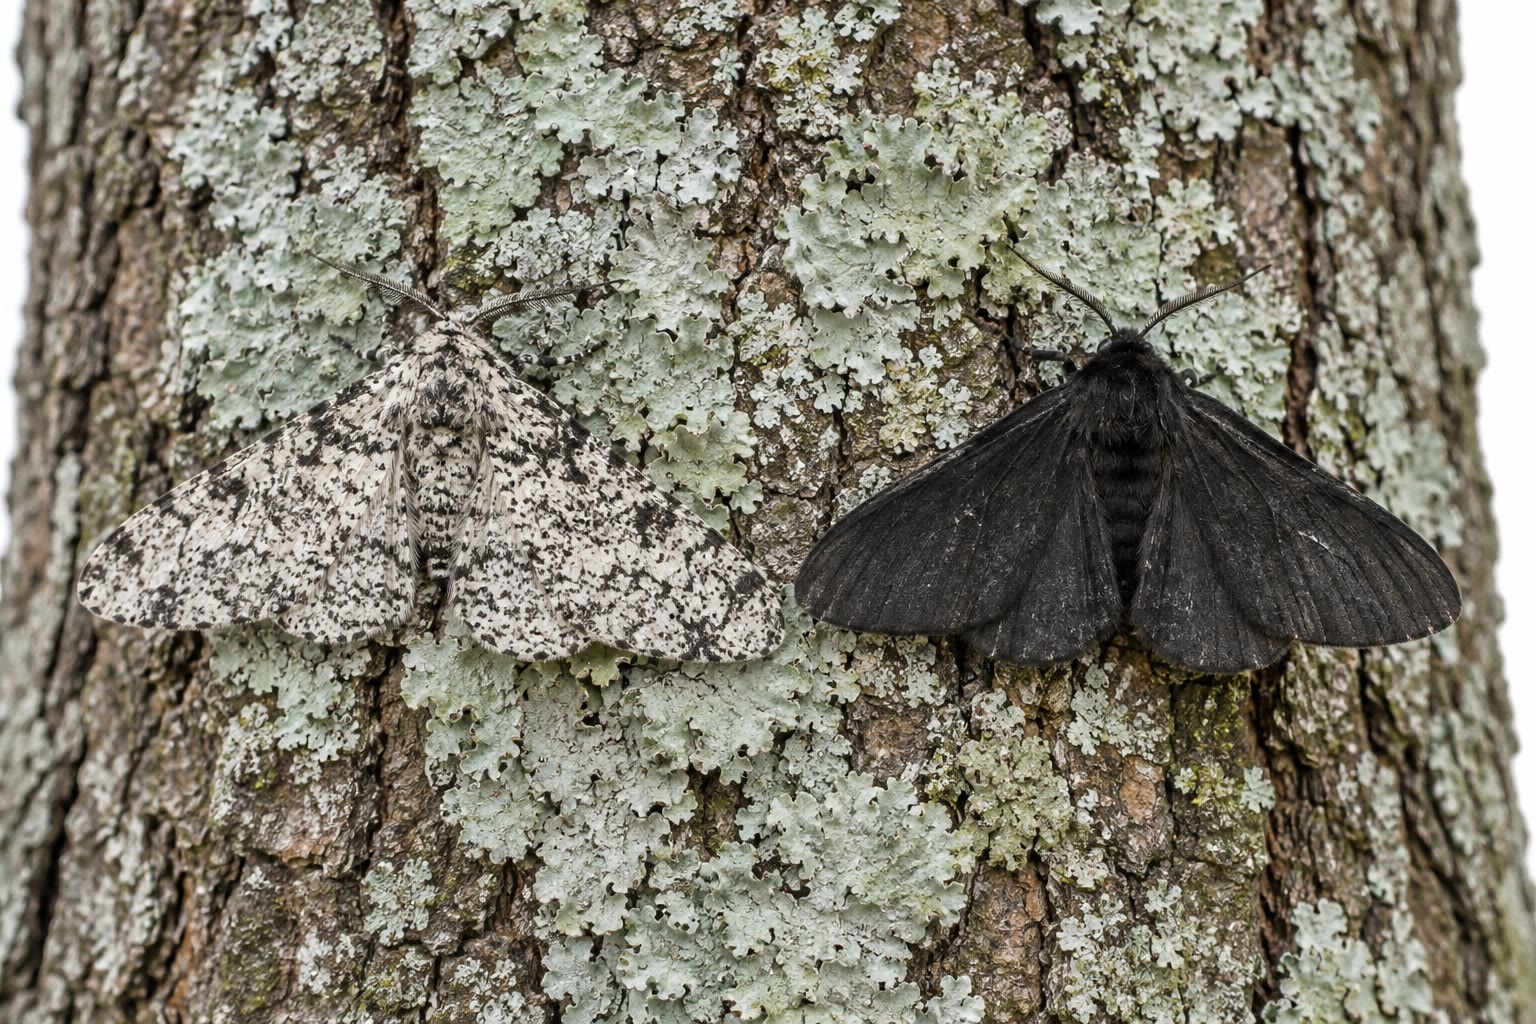
\includegraphics[width=0.46\linewidth]{images/book4/ai/b4-22-peppered-moths.jpg}\hspace{0.04\linewidth}
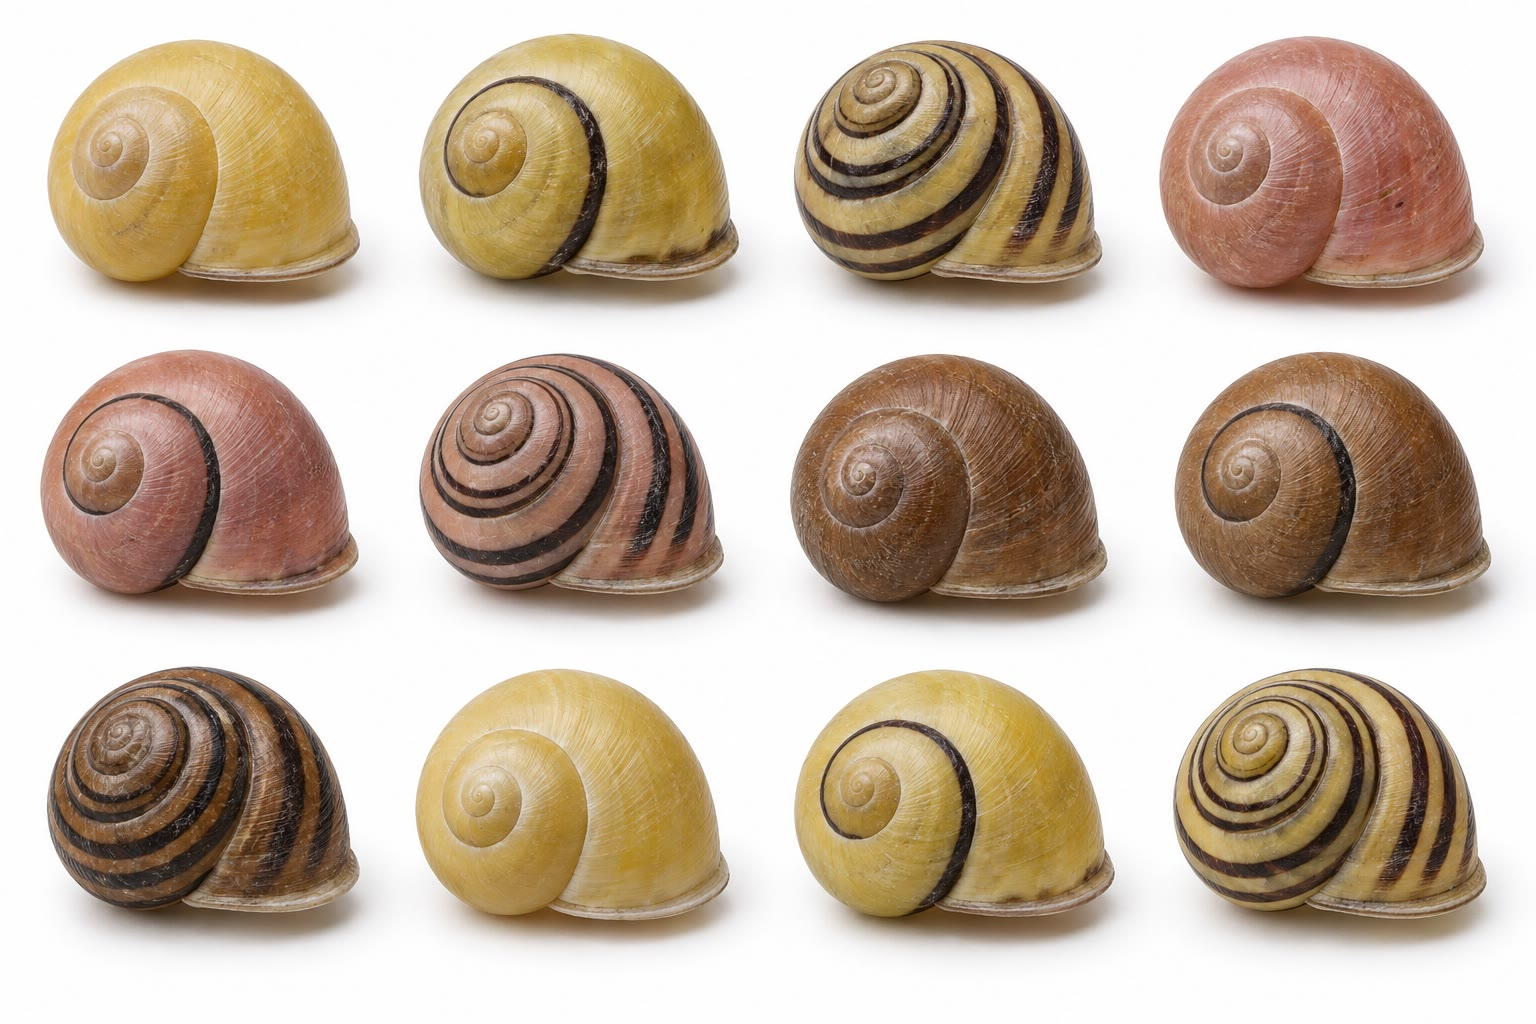
\includegraphics[width=0.46\linewidth]{images/book4/ai/b4-22-banded-snails.jpg}

{\small À gauche~: les deux formes de la phalène du bouleau sur des
lichens --- celle que trouve un oiseau dépend de l'\omterm{def:b2:plant-meristems:wood}{écorce}. À droite~: le
polymorphisme de la coquille de l'escargot des bois, couleurs et bandes
maintenues dans chaque population par des prédateurs qui apprennent à
reconnaître la forme commune.}
\end{omfigure}

\section{Exercices}

\begin{exercise}[$\star$]\label{exo:b2:population-genetics:1}
Dans un échantillon de 1000 personnes, 640 sont $MM$, 320 $MN$ et 40 $NN$.
Calculer les \omterm{def:b2:population-genetics:frequencies}{fréquences alléliques} et les effectifs attendus sous
Hardy--Weinberg. La population est-elle à l'équilibre~?
\end{exercise}

\begin{exercise}[$\star$]\label{exo:b2:population-genetics:2}
L'albinisme est \omterm{def:b2:meiosis-heredity:vocabulary}{récessif} et touche une personne sur \num{20000}.
Calculer la \omterm{def:b2:population-genetics:frequencies}{fréquence allélique} et la fréquence des porteurs.
\end{exercise}

\begin{exercise}[$\star$]\label{exo:b2:population-genetics:3}
Définir \omterm{def:b2:population-genetics:fitness}{valeur sélective}, \omterm{def:b2:population-genetics:fitness}{coefficient de sélection} et héritabilité, et
donner les cinq forces qui modifient les \omterm{def:b2:population-genetics:frequencies}{fréquences alléliques}.
\end{exercise}

\begin{exercise}[$\star$]\label{exo:b2:population-genetics:4}
Donner un exemple de \omterm{prop:b2:population-genetics:kinds}{sélection directionnelle}, un de \omterm{prop:b2:population-genetics:kinds}{sélection
stabilisante} et un de \omterm{prop:b2:population-genetics:kinds}{sélection balancée}, avec l'agent de la sélection
dans chaque cas.
\end{exercise}

\begin{exercise}[$\star\star$]\label{exo:b2:population-genetics:5}
Un \omterm{def:b2:meiosis-heredity:vocabulary}{allèle} \omterm{def:b2:meiosis-heredity:vocabulary}{récessif} létal a une fréquence de $0.02$. Combien de
générations faut-il pour la diviser par deux~? Pour atteindre $0.001$~?
Qu'est-ce que cela dit de l'effet d'empêcher les individus atteints de
se reproduire~?
\end{exercise}

\begin{exercise}[$\star\star$]\label{exo:b2:population-genetics:6}
Avec $w_{AA} = 1$, $w_{Aa} = 1$, $w_{aa} = 0.8$ et $p = 0.3$, calculer
$\bar w$, $p'$ et $\Delta p$. Recommencer pour $p = 0.9$. Pourquoi la
seconde variation est-elle tellement plus petite~?
\end{exercise}

\begin{exercise}[$\star\star$]\label{exo:b2:population-genetics:7}
Dans une région impaludée, l'\omterm{def:b2:meiosis-heredity:vocabulary}{homozygote} drépanocytaire a $w = 0.2$ et
l'\omterm{def:b2:meiosis-heredity:vocabulary}{homozygote} normal
$w = 0.88$, les \omterm{def:b2:meiosis-heredity:vocabulary}{hétérozygotes} $w = 1$. Calculer la fréquence d'équilibre
de l'\omterm{def:b2:meiosis-heredity:vocabulary}{allèle} drépanocytaire et la fraction des enfants qui naissent
malades à l'équilibre.
\end{exercise}

\begin{exercise}[$\star\star$]\label{exo:b2:population-genetics:8}
Un létal \omterm{def:b2:meiosis-heredity:vocabulary}{récessif} apparaît par \omterm{def:b2:genome-diversification:mutation}{mutation} au taux $\mu = \qty{2e-5}{}$ par
gamète. Calculer sa fréquence d'équilibre et la fraction des naissances
atteintes. Un létal \omterm{def:b2:meiosis-heredity:vocabulary}{dominant} (avant la reproduction) au même taux~:
quelle fraction des naissances~?
\end{exercise}

\begin{exercise}[$\star\star$]\label{exo:b2:population-genetics:9}
Une population de 50 reproducteurs part de $H = 0.5$.
Calculer son hétérozygotie après 10, 50 et 200 générations. Quelle doit
être la taille d'une population pour conserver \qty{90}{\%} de son
hétérozygotie sur 100 générations~?
\end{exercise}

\begin{exercise}[$\star\star\star$]\label{exo:b2:population-genetics:10}
Une île est colonisée par 10 oiseaux venus d'une population continentale
dans laquelle un \omterm{def:b2:meiosis-heredity:vocabulary}{allèle} a la fréquence $0.1$. Calculer la probabilité que
l'\omterm{def:b2:meiosis-heredity:vocabulary}{allèle} soit absent chez les fondateurs, et la probabilité qu'il soit
finalement fixé sur l'île s'il y est présent en une copie. Comparer avec
le continent.
\end{exercise}

\begin{exercise}[$\star\star\star$]\label{exo:b2:population-genetics:11}
La production laitière a une héritabilité $h^{2} = 0.3$ et un écart-type de
\qty{1000}{L}. Un éleveur garde comme mères les \qty{20}{\%} meilleures
vaches (leur moyenne est $1.4$ écart-type au-dessus de celle du troupeau).
Calculer la réponse par génération. Si les taureaux sont choisis parmi le
\qty{1}{\%} meilleur (moyenne $2.7$ écarts-types au-dessus), quelle est
la réponse~? Pourquoi la réponse ralentit-elle au bout de nombreuses
générations~?
\end{exercise}

\begin{exercise}[$\star\star\star$]\label{exo:b2:population-genetics:12}
«~La sélection est aveugle à ce qu'elle ne voit pas.~» Discuter, à
l'aide de l'\omterm{def:b2:meiosis-heredity:vocabulary}{allèle} \omterm{def:b2:meiosis-heredity:vocabulary}{récessif} chez les \omterm{def:b2:meiosis-heredity:vocabulary}{hétérozygotes}, de la \omterm{def:b2:genome-diversification:mutation}{mutation}
neutre et du caractère d'héritabilité nulle, ce sur quoi la sélection
peut et ne peut pas agir.
\end{exercise}

\section{Problème~: la phalène, l'île et le troupeau}

\begin{problem}[{Problème du week-end --- l'essor de la phalène du bouleau
calculé à partir de l'équation de la sélection, la dérive et la
consanguinité d'une population fondatrice suivies, un équilibre
mutation--sélection établi et un programme d'amélioration prédit,
jusqu'au coefficient de sélection de la phalène, à l'hétérozygotie de
l'île et au gain du troupeau}]
\label{pb:b2:population-genetics:1}
Phalène du bouleau~: \omterm{def:b2:meiosis-heredity:vocabulary}{allèle} mélanique $M$ \omterm{def:b2:meiosis-heredity:vocabulary}{dominant}, de fréquence $p_0 = 0.001$
en 1848~; \qty{90}{\%} de phalènes mélaniques 50 générations plus tard~;
on suppose
$w_{MM} = w_{Mm} = 1$ et $w_{mm} = 1 - s$. Île~: fondée par 12
oiseaux venus d'un continent où $H = 0.4$ et où un \omterm{def:b2:meiosis-heredity:vocabulary}{allèle} \omterm{def:b2:meiosis-heredity:vocabulary}{récessif}
délétère a $q = 0.05$~; l'île compte ensuite 40 oiseaux
reproducteurs. \omterm{def:b2:genome-diversification:mutation}{Mutation}~: $\mu = \qty{1e-5}{}$. Troupeau~: $h^{2} = 0.4$,
écart-type \qty{800}{L}.

\medskip
\noindent\textbf{Partie I --- La phalène.}
\begin{enumerate}
  \item En 1848, quelle fraction des phalènes était mélanique, et quelle
        fraction des \omterm{def:b2:meiosis-heredity:vocabulary}{allèles} $M$ se trouvait chez des \omterm{def:b2:meiosis-heredity:vocabulary}{hétérozygotes}~?
  \item Montrer que, $M$ étant \omterm{def:b2:meiosis-heredity:vocabulary}{dominant}, la fréquence de l'\omterm{def:b2:meiosis-heredity:vocabulary}{allèle} clair
        obéit à $q' = q(1 - sq)/(1 - sq^{2})$.
  \item En partant de $q_0 = 0.999$, calculer $q$ après une génération
        pour $s = 0.3$.
  \item \qty{90}{\%} de mélaniques signifie $q^{2} = 0.1$. Que vaut alors $q$~?
  \item Par essais successifs avec la relation de récurrence (ou
        l'approximation
        $\Delta q \approx -sq^{2}p$ tant que $q$ est voisin de 1), estimer le
        nombre de générations nécessaires, pour $s = 0.3$, pour faire
        passer $q$ de $0.999$
        à $0.32$, et comparer aux 50 observées.
  \item Après les lois sur la qualité de l'air, la forme claire a
        l'avantage~: $s
        = 0.3$ contre $mm$ devient $s = 0.3$ contre $M\_$. Montrer
        que $\Delta p = -spq^{2}/\bar w$, et expliquer pourquoi le retour
        de la forme claire est d'abord lent et se termine par un déclin
        exponentiel de $M$, alors que l'essor avait commencé de façon
        exponentielle et s'était terminé par une lente reptation.
\end{enumerate}

\medskip
\noindent\textbf{Partie II --- L'île.}
\begin{enumerate}[resume]
  \item Calculer la probabilité qu'aucun des 12 fondateurs ne porte
        l'\omterm{def:b2:meiosis-heredity:vocabulary}{allèle} délétère.
  \item Calculer l'hétérozygotie attendue après la génération fondatrice
        (tirée de $H = 0.4$ par 12 individus, soit 24
        copies de gènes).
  \item Calculer l'hétérozygotie après 100 générations avec $N =
        40$, en fraction de celle du continent.
  \item Une \omterm{def:b2:genome-diversification:mutation}{mutation} neutre apparaît chez un oiseau. Calculer sa
        probabilité de fixation et le temps attendu jusqu'à la fixation
        si elle se fixe.
  \item Les oiseaux de l'île s'accouplent au hasard mais sont tous
        apparentés. Avec
        $F = 1/(2N)$ s'accumulant à chaque génération jusqu'à environ $0.3$ après
        30 générations, calculer la fréquence des \omterm{def:b2:meiosis-heredity:vocabulary}{homozygotes} atteints
        pour l'\omterm{def:b2:meiosis-heredity:vocabulary}{allèle} à $q = 0.05$, avec et sans consanguinité.
  \item Un oiseau du continent arrive à chaque génération. Expliquer
        l'effet sur la divergence de l'île et sur son fardeau.
\end{enumerate}

\medskip
\noindent\textbf{Partie III --- L'équilibre.}
\begin{enumerate}[resume]
  \item Calculer la fréquence d'équilibre d'un \omterm{def:b2:meiosis-heredity:vocabulary}{récessif} létal alimenté
        par $\mu = 10^{-5}$, et la fraction des naissances atteintes.
  \item Faire le même calcul pour $s = 0.1$ (un \omterm{def:b2:meiosis-heredity:vocabulary}{récessif} légèrement
        délétère).
  \item Calculer l'équilibre d'un \omterm{def:b2:meiosis-heredity:vocabulary}{allèle} \omterm{def:b2:meiosis-heredity:vocabulary}{dominant} de désavantage
        \omterm{def:b2:meiosis-heredity:vocabulary}{hétérozygote} $hs = 0.05$.
  \item La médecine soigne le létal, si bien que $s$ tombe à $0.1$.
        Comment l'équilibre change-t-il, et combien de temps (ordre de
        grandeur) la population met-elle pour l'atteindre~?
  \item Le génome compte \num{20000} gènes, chacun mutant vers un
        \omterm{def:b2:meiosis-heredity:vocabulary}{récessif} létal au taux $10^{-5}$. Combien d'\omterm{def:b2:meiosis-heredity:vocabulary}{allèles} létaux une
        personne moyenne porte-t-elle à l'état \omterm{def:b2:meiosis-heredity:vocabulary}{hétérozygote}~? (À
        l'équilibre, chaque locus compte $2\hat q$ copies par personne.)
  \item Expliquer pourquoi ce nombre est compatible avec une population
        en bonne santé et pourquoi il rend coûteux les mariages entre cousins.
\end{enumerate}

\medskip
\noindent\textbf{Partie IV --- Le troupeau.}
\begin{enumerate}[resume]
  \item L'éleveur garde les \qty{30}{\%} meilleures vaches (moyenne $1.16$
        écart-type au-dessus du troupeau). Calculer la différentielle
        de sélection en litres et la réponse.
  \item Après cinq générations de la même sélection, quel est le gain
        attendu, et pourquoi le gain réel pourrait-il être plus faible~?
  \item Les taureaux apportent la moitié des gènes et sont choisis parmi
        les \qty{2}{\%} meilleurs ($2.4$ écarts-types). Calculer la réponse
        lorsque vaches et taureaux sont sélectionnés comme ci-dessus
        (faire la moyenne des deux différentielles).
  \item Un troupeau dont toutes les vaches sont des \omterm{def:b2:asexual-reproduction:clone}{clones} d'un même
        animal~: que valent
        $h^{2}$ et la réponse~? Qu'est-ce que cela dit de l'héritabilité~?
  \item Une population de pinsons a une héritabilité $h^{2} = 0.7$ pour la
        hauteur du bec, et la sécheresse laisse des survivants au bec plus
        haut de \qty{0.6}{mm}. Prévoir la génération suivante.
  \item L'éleveur passe à un caractère d'héritabilité $h^{2} = 0.1$.
        Quelle différentielle de sélection, en écarts-types, donne la
        même réponse qu'à la question 19~?
  \item Énoncer le résultat~: le $s$ de la phalène et le temps nécessaire
        pour atteindre \qty{90}{\%} de mélaniques, l'hétérozygotie de
        l'île après 100 générations, et la réponse du troupeau par
        génération.
\end{enumerate}
\end{problem}
